\graphicspath{{Introduction/figures/}}
\chapter{Introduction}\label{ch:intro}
%\thispagestyle{empty}

\runningchaptertitle{Introduction}
%\bstctlcite{IEEE:BSTcontrol}
%% Use this code to put your background image
%\ThisCenterWallPaper{\wpScaling}{ChapterBackground.png}
%\noabstract
\ThumbIndexShow

\newcommand{\tb}{\textit{{\textbf{}}}}



\section{Pulmonary anatomy}

The human lungs consist of a left lung and right lung, as shown in Figure \ref{fig:lobes}. The right and left lung anatomy are similar but asymmetrical. Each lung is composed of smaller units called lobes. Each lung is divided into lobes by the fissures. The right lung has two fissures; the horizontal and oblique fissures, and three lobes, namely the right upper lobe (RUL), the right middle lobe (RML), and the right lower lobe (RLL). There are two lobes, the left upper lobe (LUL) and the left lower lobe (LLL), divided by the oblique fissure in the left lung \cite{aung2019overview}.



\begin{figure}
    \centering
    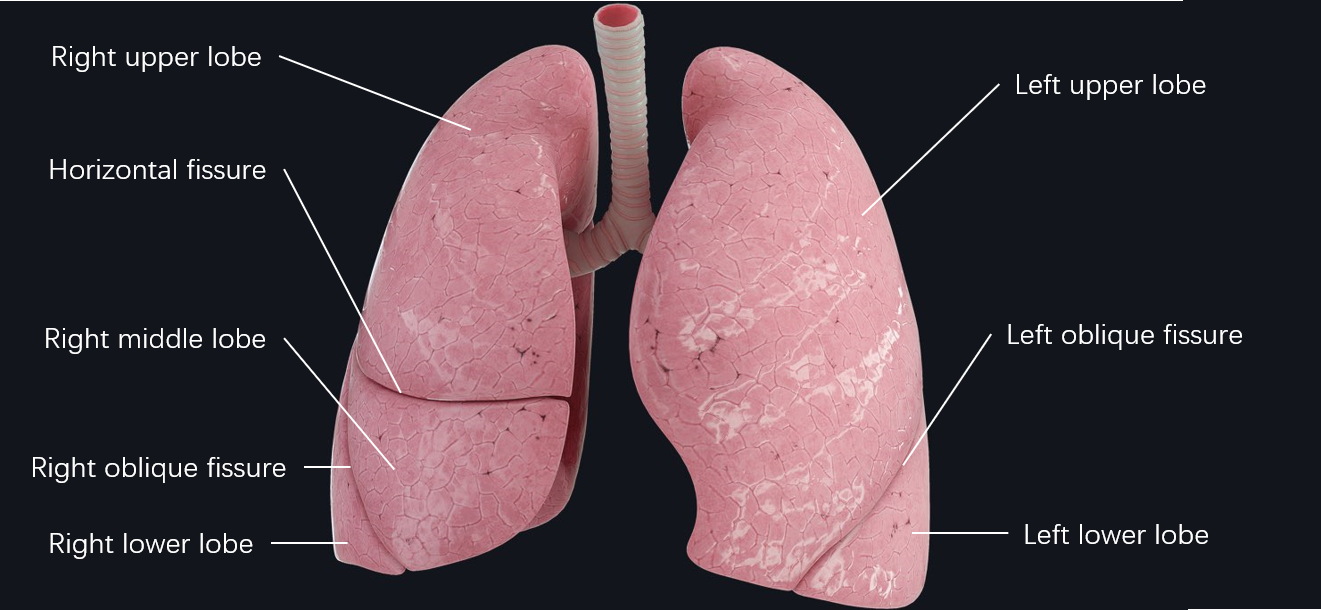
\includegraphics[width=0.7\linewidth]{Introduction/figures/lobes.png}
    \caption{Lung lobes (modified and adopted from \url{https://3d4medical.com/blog/auscultation-of-the-lungs}).}
    \label{fig:lobes}
\end{figure}


\begin{figure}
    \centering
    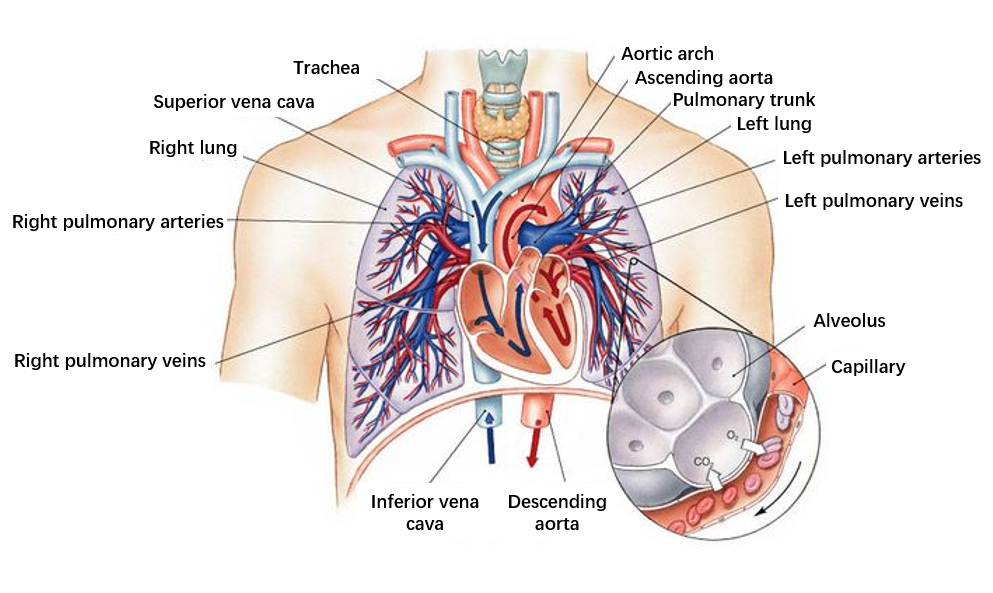
\includegraphics[width=0.7\linewidth]{Introduction/figures/lung.png}
    \caption{Pulmonary circulation (modified and adopted from \url{https://3d4medical.com/blog/auscultation-of-the-lungs}).}
    \label{fig:lung}
\end{figure}

The major function of the lungs is to perform gas exchange, which requires blood from the pulmonary circulation. This blood supply contains deoxygenated blood and travels to the lungs where erythrocytes, also known as red blood cells, pick up oxygen to be transported to tissues throughout the body \cite{aung2019overview}. The pulmonary artery is an artery that arises from the pulmonary trunk and carries deoxygenated, arterial blood to the alveoli. The pulmonary artery branches multiple times as it follows the bronchi, and each branch becomes progressively smaller in diameter. One arteriole and an accompanying venule supply and drain one pulmonary lobule. As they near the alveoli, the pulmonary arteries become the pulmonary capillary network. The pulmonary capillary network consists of tiny vessels with very thin walls that lack smooth muscle fibers. The capillaries branch and follow the bronchioles and structure of the alveoli. It is at this point that the capillary wall meets the alveolar wall, creating the respiratory membrane. Once the blood is oxygenated, it drains from the alveoli by way of multiple pulmonary veins, which exit the lungs through the hilum \cite{aung2019overview, martini2005anatomy}.

\section{Systemic sclerosis}
Systemic sclerosis (SSc) is an immune-mediated rheumatic disease that is characterised by aberrant immune activation, vascular injury followed by defective neovascularization and impaired remodeling, and extensive tissue fibrosis of the skin and certain internal organs \cite{denton2017systemic,asano2018systemic}. Although systemic sclerosis is uncommon, it has a high morbidity — greater than any other rheumatic disease \cite{denton2017systemic}.   Lung fibrosis or interstitial lung disease (ILD) is the primary contribuor of death, followed by Pulmonary arterial hypertension (PAH) and cardiac causes  \cite{Acharya2013, steele2012clinical}. ILD is present in 80\% of patients with systemic sclerosis \cite{codes2023systemic}. The heterogeneous expression of this rare disease poses challenges to both the patient and clinician, particularly with regard to predicting the development of serious internal organ involvement. Although early and accurate diagnosis and classification might improve patient outcomes, clinicians often struggle to diagnose systemic sclerosis early in the disease course \cite{volkmann2023systemic}.  Screening strategies facilitate timely recognition of life-threatening complications and initiation of targeted therapies to halt their progression \cite{allanore2015systemic}.

The main tools to diagnosis SSc related ILD (SSc-ILD) include \textbf{pulmonary function tests (PFTs)} and chest\textbf{ high resolution computed tomography (HRCT) }scans \cite{codes2023systemic}. Although PFTs are central to monitoring interstitial lung disease progression, they have limited sensitivity in diagnosing interstitial lung disease \cite{bernstein2020performance}. PFTs are associated with intraindividual variation during repeated measurements and extrapulmonary factors (e.g., oral fibrosis, thoracic fibrosis, myopathy, fatigue, and cachexia) can influence the results. Proposed definitions of progressive interstitial lung disease based on PFT and HRCT trends can help identify patients with a progressive fibrosing phenotype who could benefit from more aggressive or alternate therapies \cite{distler2020predictors}. A clinical practice guideline defined progressive pulmonary fibrosis as fulfilling at least two of three criteria (worsening symptoms, radiological progression, and physiological progression) within the past year with no alternative explanation in a patient with an interstitial lung disease other than idiopathic pulmonary fibrosis. Involvement of experienced thoracic radiologists is central to identifying more subtle progression of interstitial lung disease on HRCT \cite{raghu2022idiopathic}. Invasive procedures, including both bronchoalveolar lavage and lung biopsy, are typically only done in cases of diagnostic uncertainty. 

\section{Pulmonary function tests}

To evaluate progression of SSc-ILD, various pulmonary function tests (PFTs) are used as key measures \cite{Behr2008, Caron2018, Ninaber2015}, such as the diffusion capacity for carbon monoxide (DLCO), forced expiratory volume in 1 second (FEV\textsubscript{1}), forced vital capacity (FVC) and total lung capacity (TLC). 

\begin{itemize} 
\item DLCO. DLCO is a measurement to assess the lungs' ability to transfer gas from inspired air to the bloodstream \cite{Graham2017} (see Figure \ref{fig:chap1_dlco}). Carbon monoxide (CO) is used for this test because it has a higher affinity for hemoglobin (200 to 250 times that of oxygen), and it follows the same pathway as that of oxygen to finally bind with hemoglobin. Oxygen is not preferred since its uptake is limited by cardiac uptake and total body consumption \cite{mehra2017evaluation}. DLCO is expressed as mL/min/mm Hg, represents mL of CO transferred per minute for each mm Hg of pressure difference across the total available functioning lung gas exchange surface \cite{macintyre2005standardisation}. 

\item FEV\textsubscript{1}. FEV\textsubscript{1} is the amount of air exhaled during the first second of the FVC maneuver (Figure \ref{fig:chap1_pft}). It tends to be lower in diseases that obstruct the airway, such as asthma or emphysema.

\item FVC. A breathing curve begins with the patient inhaling as deeply as he or she can. Then the patient exhales as long and as forcefully as possible; the amount exhaled in this manner is the FVC (Figure \ref{fig:chap1_pft}).

\item TLC. Even after one exhales as long and as hard as possible, some air remains in the lungs; this is called the residual volume (RV). The residual volume plus the FVC equals the TLC (see Figure \ref{fig:chap1_pft}). The RV (and hence the TLC) cannot be measured by spirometry. Rather, they must be measured by special tests that require the patient either to breathe an inert gas such as helium (the concentration of which is measured in the expired air, from which the residual volume is calculated) or to sit in an airtight booth in which the pressure is measured as he or she breathes. 

\end{itemize}



\begin{figure}[tb]
    \centering
    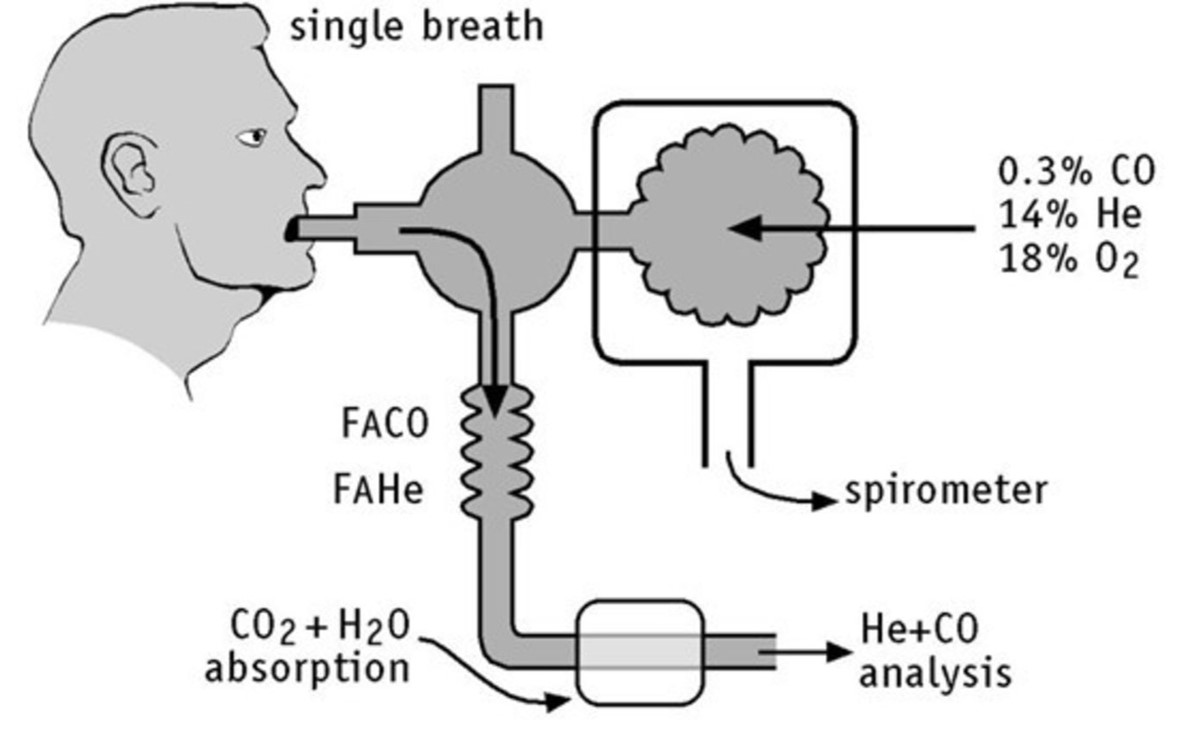
\includegraphics[width=0.6\textwidth]{Introduction/figures/dlco.jpg}
    \caption{Illustration of DLCO measurement. FACO: Fraction of Carbon Monoxide in Alveolar Gas. FAHE: Fraction of Helium in Alveolar Gas. (adopted from \cite{Sylvester2020}).}
    \label{fig:chap1_dlco}
\end{figure}




\begin{figure}[tb]
    \centering
    
\includegraphics[width=0.8\textwidth]{Introduction/figures/PFTs.png}
    \caption{Breathing curve measured by spirometry. RV: residual volume, FEV\textsubscript{1}: forced expiratory volume in 1 second, FVC: forced vital capacity, TLC: total lung capacity (adopted and modified from \url{https://bronchiectasis.com.au/bronchiectasis/diagnosis-2/lung-function}).}
    \label{fig:chap1_pft}
\end{figure}



PFTs can, however, not always be performed if there is a risk of disease transmission, e.g. in patients with COVID-19, active tuberculosis or other airborne infectious diseases \cite{choi2022automated, McGowan2022}. In addition, some patients, who have hemoptysis or had surgery in the past month, or other contraindications \cite{Cooper, Meng2023}, like aneurysmatic abnormalities and ischaemic stroke, are not able to perform PFTs because the forced exhalation during spirometry may increase the risk of complications [9].

\section{Chest CT}
According to expert consensus, PFTs should be ordered in all patients with SSc and repeated regularly to monitor the progress of SSc \cite{hoffmann2020identification}. However, some patients with SSc, particularly those with anti-topoisomerase antibodies, have normal FVC and DLCO values despite the presence of fibrosis on computed tomography (CT) \cite{showalter2018performance}. Therefore, CT also plays an import role on the accurate diagnosis of SSc.

CT, as a non-invasive imaging technique, is the gold standard for the detection of ILD in SSc disease \cite{codes2023systemic}. A chest CT scan offers a more intricate visualization compared to a standard chest X-ray. It captures multiple views of the lungs, which are then combined into three-dimensional, cross-sectional representations, visualizing the organs' dimensions, contours, and internal architecture. CT could provide valuable findings including the pattern of ILD (e.g. ground glass opacity and reticulation shown in Figure \ref{fig:chap1_ct_samples}) and the severity or extent of fibrosis, findings that correlate with disease prognosis \cite{silver2015management}. Expert consensus guidelines recommend that CT should be performed in all SSc patients to screen for ILD \cite{hoffmann2020identification}.

\begin{figure}[tb]
    \centering
    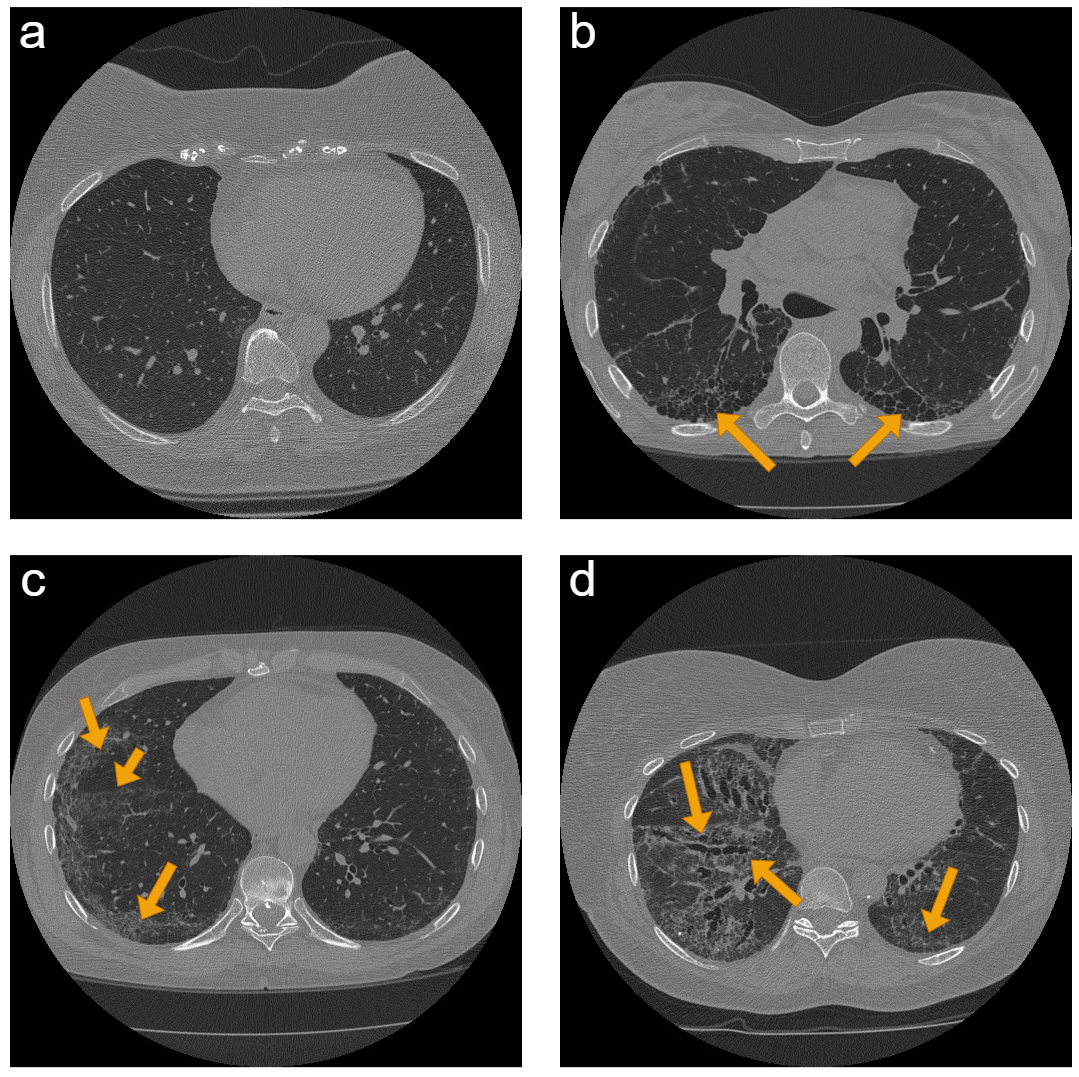
\includegraphics[width=0.8\textwidth]{Introduction/figures/ct_samples.png}
    \caption{Slices of CT scans from a SSc patient with different patterns (arrows). a) normal case, b) with reticulation pattern, c) with ground glass opacity pattern, d) with reticulation and ground glass opacity pattern pattern.}
    \label{fig:chap1_ct_samples}
\end{figure}



\section{Deep learning on chest CT}

Although high-resolution CT scans could provide detailed information, there are still some challenges for the diagnosis of lung disease from CT scans. For example, 1) pixel-wise object segmentation is normally a necessary step for subsequent diagnosis but it is laborious for human experts; 2) Visual severity estimation is subjective and significantly rely on the experience of clinicians; 3) A high-resolution CT normally include more than 500 slices, which significantly increase the diagnostic workload for clinicians. In order to overcome such challenges for the analysis of chest CT images, deep learning techniques were introduced to automate 

Deep learning could be divided to supervised learning, unsupervised learning,  semi-supervised learning, and weakly supervised learning. Typically, the deep learning models are trained using labeled data, called supervised learning. However, for tasks where manually generating labels is laborious and expensive, the use of unsupervised learning methods is of significant value \cite{hussein2019lung}. Unsupervised learning tries to reveal the structure within the data on its own \cite{liang2020model}. Semi-supervised learning utilizes both labeled and unlabeled data. Weakly supervised learning tried to achieve the learning with coarse-grained labels or inaccurate labels \cite{zhou2018brief}.

Deep learning models could be applied for classification (e.g. classification of ), segmentation (e.g. segmentation of lungs \cite{skourt2018lung, yoo2021automated}, lobes \cite{Jia2021}, Covid-19 lesions \cite{saood2021covid}, nodules \cite{wu2019survey}), regression (e.g. regression of severity score\cite{Jia2022}, pulmonary function tests \cite{jia2023automatic}), detection (e.g. detection of lung cancer \cite{shakeel2019lung}), reconstruction (e.g. low-dose CT reconstruction\cite{liang2020model}), registration (e.g. iter-patient registration \cite{de2019deep}), etc. 

\section{Thesis outline}

The aim of this thesis is to develop these methods focusing on quantifying disease sevirity of SSc disease based on CT images. The research topics and connections between each chapter are summarized in Figure \ref{fig:overview}. 

\begin{figure}[tb]
    \centering
    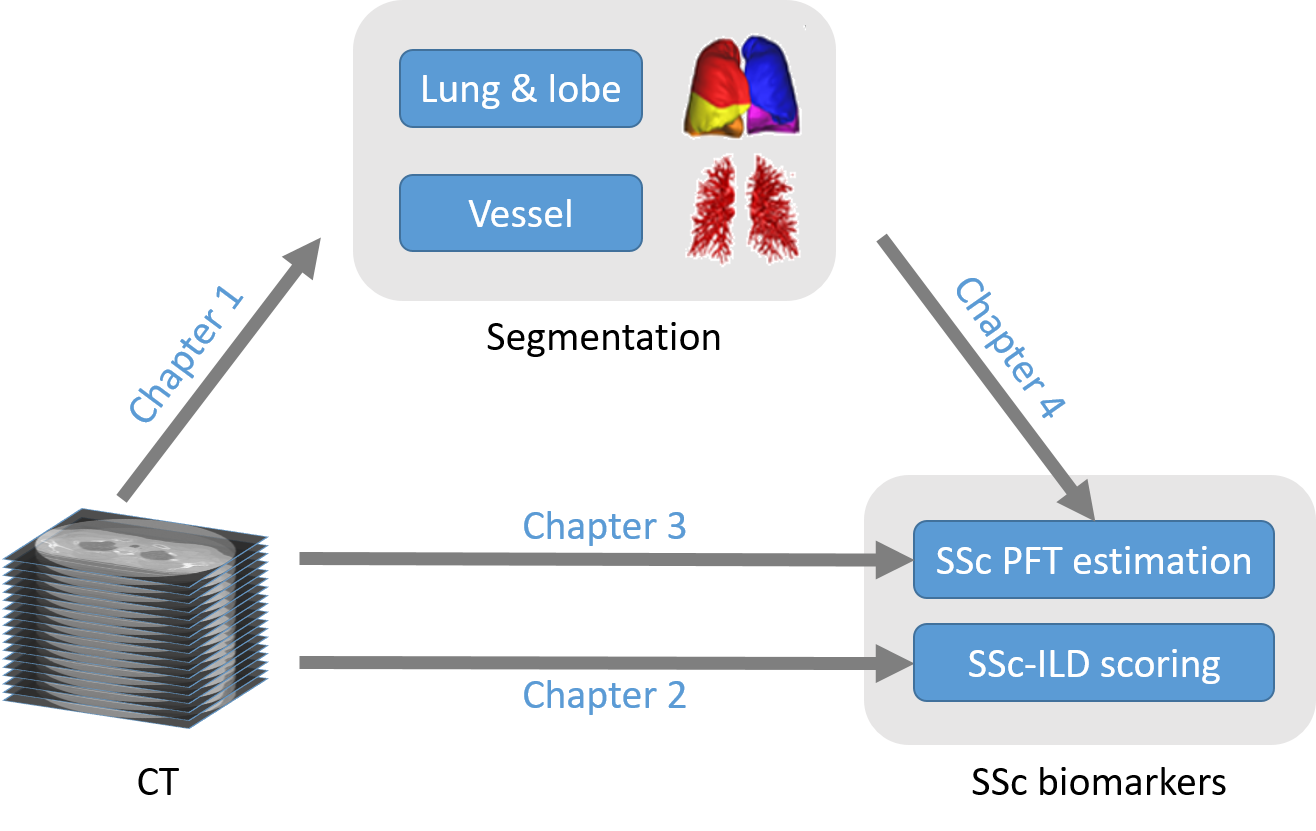
\includegraphics[width=0.8\textwidth]{Introduction/figures/outline.png}
    \caption{Overview of the research topics in this thesis.}
    \label{fig:overview}
\end{figure}


%\begin{description}[align=left]
\textbf{Chapter 2} developed a deep learning based network for lobe segmentation. We proposed a multi-task semi-supervised model that can leverage information of multiple structures from unannotated datasets and datasets annotated with different structures. A focused alternating training strategy is presented to balance the different tasks. We evaluated the trained model on an external independent CT dataset. The results show that our model significantly outperforms single-task alternatives. We also demonstrated that our approach is successful for different network architectures as backbones. 

\textbf{Chapter 3} developed a deep learning framework to automate SSc-ILD scoring. The automated framework is a cascade of two neural networks. The first network selects the craniocaudal positions of the five scoring levels. Subsequently, for each level, the second network estimates the ratio of three patterns to the total lung area: the total extent of disease (TOT), ground glass (GG) and reticulation (RET). To overcome the score imbalance in the second network, we propose a method to augment the training dataset with synthetic data. To explain the network’s output, a heat map method is introduced to highlight the candidate interstitial lung disease regions. The results show our framework performs competitively with human experts and provides high-quality explanations using heat maps.

\textbf{Chapter 4} proposed a deep learning based framework to automatically estimate PFT results from chest CT scans of SSc patients. We use segmented lungs and vessels to mask the CT images seperately to explore how different regions influence the estimation of pulmonary function tests (PFTs). We also proposed regression attention maps (RAM), which showed the contribution of different regions. This suggests that that manually designed imaging biomarkers can still contribute to explaining the relation between lung function and structure.

\textbf{Chapter 5} extended the work of \textbf{Chapter 4} to improve PFTs estimation performance. We developed a point cloud neural network (PNN-Vessel) and graph neural network (GNN-Vessel), based on the point cloud data and graph data of centerlines, respectively. The results show that both PNN-Vessel and GNN-Vessel could outperform CNN-Vessel (CNN network developed on 3D grid vessel masks). It verified that more detailed vessel information could provide more explanation of PFTs estimation. By combining CNN-CT (CNN network developed on 3D CT), PNN-Vessel and GNN-Vessel, we could achieve the best PFTs estimation performance.

\textbf{Chapter 6} summarizes and discusses the overall achievements of this thesis.

%\end{description} 
